\documentclass[tikz,border=7pt]{standalone}
\usepackage{amsmath,amssymb}
\usetikzlibrary{arrows.meta,positioning,calc,fit,backgrounds}

\definecolor{Ink}{HTML}{23384D}
\definecolor{Muted}{HTML}{607487}
\definecolor{Guide}{HTML}{D9E1E7}
\definecolor{TravelBlue}{HTML}{315F8C}
\definecolor{AutoTeal}{HTML}{3E7773}
\definecolor{RoadAmber}{HTML}{A66C32}
\definecolor{RailBlue}{HTML}{496A9B}
\definecolor{OutsideGray}{HTML}{707982}

\tikzset{
	font=\sffamily,
	major/.style={-{Stealth[length=2.25mm,width=1.55mm]}, draw=Ink!88,
		line width=0.96pt, rounded corners=1.4pt, line cap=round, line join=round},
	choice/.style={-{Stealth[length=1.95mm,width=1.32mm]}, draw=Ink!76,
		line width=0.74pt, rounded corners=1.3pt, line cap=round, line join=round},
	branch/.style={draw=Ink!62, line width=0.60pt, rounded corners=1.3pt,
		line cap=round, line join=round},
	root/.style={draw=Ink, line width=0.95pt, fill=white, rounded corners=2.2pt,
		minimum width=47mm, minimum height=11mm, align=center, inner sep=3pt},
	decision/.style={draw=TravelBlue, line width=0.90pt, fill=TravelBlue!7,
		rounded corners=2.2pt, minimum width=40mm, minimum height=12mm,
		align=center, inner sep=3pt},
	mode/.style={line width=0.82pt, rounded corners=2pt, minimum height=16mm,
		align=center, inner sep=3pt},
	automode/.style={mode, draw=AutoTeal, fill=AutoTeal!8, minimum width=36mm},
	roadmode/.style={mode, draw=RoadAmber, fill=RoadAmber!8, minimum width=40mm},
	railmode/.style={mode, draw=RailBlue, fill=RailBlue!8, minimum width=39mm},
	leaf/.style={line width=0.66pt, rounded corners=1.6pt, minimum height=15mm,
		align=center, inner sep=2.5pt, font=\scriptsize},
	autoleaf/.style={leaf, draw=AutoTeal!90, fill=white, text width=15mm},
	roadleaf/.style={leaf, draw=RoadAmber!90, fill=white, text width=24mm},
	productleaf/.style={leaf, draw=RailBlue!90, fill=white, text width=19mm},
	seatleaf/.style={line width=0.66pt, rounded corners=1.6pt, minimum height=13mm,
		align=center, inner sep=2pt, font=\scriptsize, draw=RailBlue!90, fill=white,
		text width=14mm},
	level/.style={fill=Ink, text=white, rounded corners=1.7pt, text width=26mm,
		minimum height=11mm, align=left, inner xsep=4pt, font=\scriptsize},
	prob/.style={fill=white, fill opacity=.96, text opacity=1, text=Ink,
		rounded corners=.8pt, inner xsep=2pt, inner ysep=1.2pt, font=\scriptsize},
	flowbox/.style={draw=Guide, line width=0.70pt, fill=Ink!2, rounded corners=2pt,
		minimum width=160mm, minimum height=24mm, align=center, inner sep=4pt},
	note/.style={font=\scriptsize, text=Muted, align=center}
}

\begin{document}
	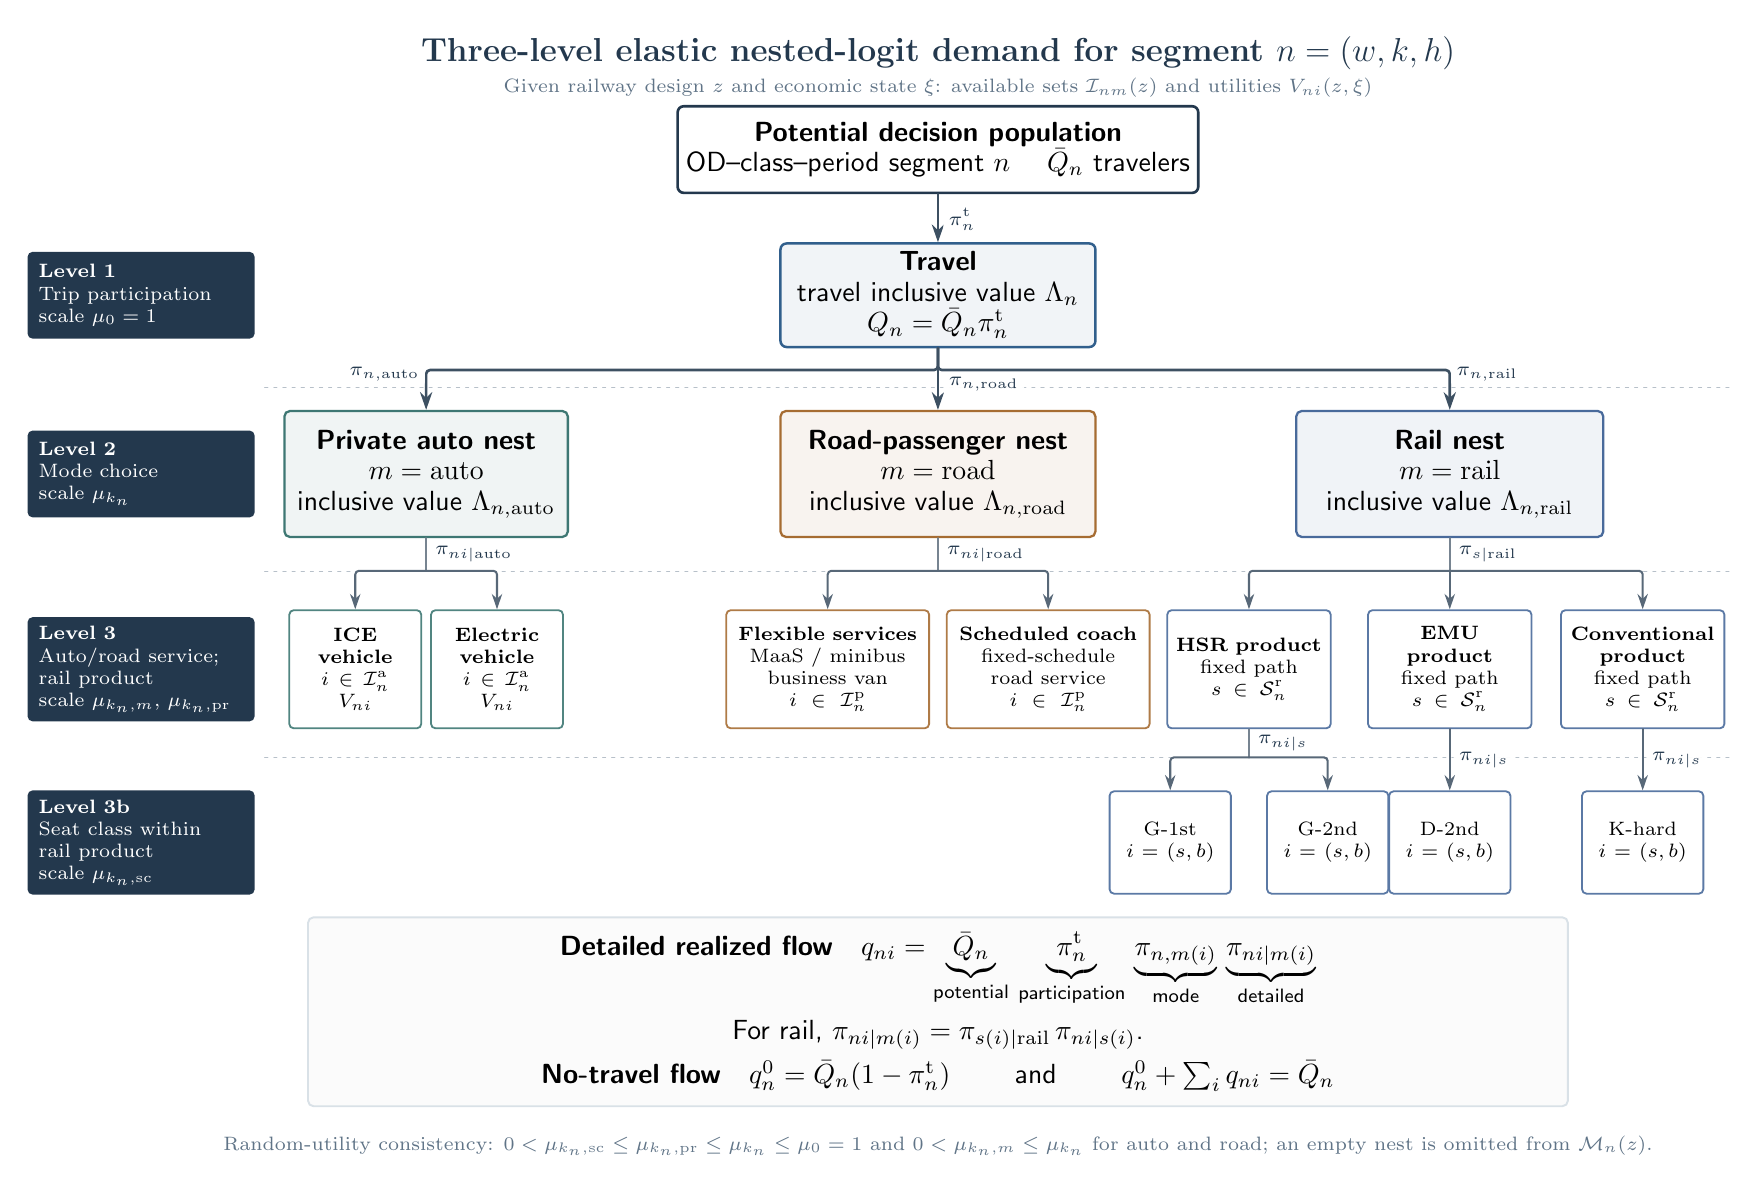
\begin{tikzpicture}[x=1cm,y=1cm]
		% Title and model inputs
		\node[font=\bfseries\large, text=Ink] at (0,1.22)
		{Three-level elastic nested-logit demand for segment $n=(w,k,h)$};
		\node[note] at (0,0.78)
		{Given railway design $z$ and economic state $\xi$: available sets $\mathcal I_{nm}(z)$ and utilities $V_{ni}(z,\xi)$};
		
		% Potential market and participation decision
		\node[root] (potential) at (0,0)
		{\textbf{Potential decision population}\\[-1pt]
			OD--class--period segment $n$ \quad $\bar Q_n$ travelers};
		
		\node[decision] (travel) at (0,-1.85)
		{\textbf{Travel}\\[-1pt]
			travel inclusive value $\Lambda_n$\\[-1pt]
			$Q_n=\bar Q_n\pi_n^{\mathrm t}$};
		
		\draw[major] (potential.south) --
		node[prob, pos=.53, right=1.5pt] {$\pi_n^{\mathrm t}$} (travel.north);
		
		% Mode nests
		\node[automode] (auto) at (-6.50,-4.12)
		{\textbf{Private auto nest}\\[-1pt]
			$m=\mathrm{auto}$\\[-1pt]
			inclusive value $\Lambda_{n,\mathrm{auto}}$};
		\node[roadmode] (road) at (0,-4.12)
		{\textbf{Road-passenger nest}\\[-1pt]
			$m=\mathrm{road}$\\[-1pt]
			inclusive value $\Lambda_{n,\mathrm{road}}$};
		\node[railmode] (rail) at (6.50,-4.12)
		{\textbf{Rail nest}\\[-1pt]
			$m=\mathrm{rail}$\\[-1pt]
			inclusive value $\Lambda_{n,\mathrm{rail}}$};
		
		\draw[major] (travel.south) -- (0,-2.80) -|
		node[prob, pos=.70, above left=0pt] {$\pi_{n,\mathrm{auto}}$} (auto.north);
		\draw[major] (travel.south) --
		node[prob, pos=.58, right=1.5pt] {$\pi_{n,\mathrm{road}}$} (road.north);
		\draw[major] (travel.south) -- (0,-2.80) -|
		node[prob, pos=.70, above right=0pt] {$\pi_{n,\mathrm{rail}}$} (rail.north);
		
		% Level 3 leaves: auto and road alternatives, and rail products
		\node[autoleaf] (ice) at (-7.40,-6.60)
		{\textbf{ICE vehicle}\\$i\in\mathcal I_n^{\mathrm a}$\\$V_{ni}$};
		\node[autoleaf] (ev) at (-5.60,-6.60)
		{\textbf{Electric vehicle}\\$i\in\mathcal I_n^{\mathrm a}$\\$V_{ni}$};
		
		\node[roadleaf] (flex) at (-1.40,-6.60)
		{\textbf{Flexible services}\\MaaS / minibus\\business van \quad $i\in\mathcal I_n^{\mathrm p}$};
		\node[roadleaf] (coach) at (1.40,-6.60)
		{\textbf{Scheduled coach}\\fixed-schedule road service\\$i\in\mathcal I_n^{\mathrm p}$};
		
		\node[productleaf] (hsr) at (3.95,-6.60)
		{\textbf{HSR product}\\fixed path\\$s\in\mathcal S^{\mathrm r}_n$};
		\node[productleaf] (emu) at (6.50,-6.60)
		{\textbf{EMU product}\\fixed path\\$s\in\mathcal S^{\mathrm r}_n$};
		\node[productleaf] (conv) at (8.95,-6.60)
		{\textbf{Conventional product}\\fixed path\\$s\in\mathcal S^{\mathrm r}_n$};
		
		% Level 3b: seat classes within each rail product
		\node[seatleaf] (g1) at (2.95,-8.80) {G-1st\\$i=(s,b)$};
		\node[seatleaf] (g2) at (4.95,-8.80) {G-2nd\\$i=(s,b)$};
		\node[seatleaf] (d2) at (6.50,-8.80) {D-2nd\\$i=(s,b)$};
		\node[seatleaf] (kh) at (8.95,-8.80) {K-hard\\$i=(s,b)$};
		
		% Orthogonal fan-outs keep probability lines clear of labels.
		\coordinate (aj) at (-6.50,-5.35);
		\coordinate (pj) at (0,-5.35);
		\coordinate (rj) at (6.50,-5.35);
		\coordinate (hj) at (3.95,-7.72);
		\draw[branch] (auto.south) --
		node[prob, pos=.48, right=1pt] {$\pi_{ni\mid\mathrm{auto}}$} (aj);
		\draw[choice] (aj) -| (ice.north);
		\draw[choice] (aj) -| (ev.north);
		
		\draw[branch] (road.south) --
		node[prob, pos=.48, right=1pt] {$\pi_{ni\mid\mathrm{road}}$} (pj);
		\draw[choice] (pj) -| (flex.north);
		\draw[choice] (pj) -| (coach.north);
		
		\draw[branch] (rail.south) --
		node[prob, pos=.48, right=1pt] {$\pi_{s\mid\mathrm{rail}}$} (rj);
		\draw[choice] (rj) -| (hsr.north);
		\draw[choice] (rj) -- (emu.north);
		\draw[choice] (rj) -| (conv.north);
		
		% Seat-class fan-outs within each product
		\draw[branch] (hsr.south) --
		node[prob, pos=.50, right=1pt] {$\pi_{ni\mid s}$} (hj);
		\draw[choice] (hj) -| (g1.north);
		\draw[choice] (hj) -| (g2.north);
		\draw[choice] (emu.south) --
		node[prob, pos=.50, right=1pt] {$\pi_{ni\mid s}$} (d2.north);
		\draw[choice] (conv.south) --
		node[prob, pos=.50, right=1pt] {$\pi_{ni\mid s}$} (kh.north);
		
		% Level labels
		\node[level] at (-10.12,-1.85)
		{\textbf{Level 1}\\Trip participation\\scale $\mu_0=1$};
		\node[level] at (-10.12,-4.12)
		{\textbf{Level 2}\\Mode choice\\scale $\mu_{k_n}$};
		\node[level] at (-10.12,-6.60)
		{\textbf{Level 3}\\Auto/road service;\\rail product\\scale $\mu_{k_n,m}$, $\mu_{k_n,\mathrm{pr}}$};
		\node[level] at (-10.12,-8.80)
		{\textbf{Level 3b}\\Seat class within\\rail product\\scale $\mu_{k_n,\mathrm{sc}}$};
		
		% Demand composition and scale ordering
		\node[flowbox] (flow) at (0,-10.95)
		{\textbf{Detailed realized flow}\quad
			$q_{ni}=\underbrace{\bar Q_n}_{\text{potential}}\,
			\underbrace{\pi_n^{\mathrm t}}_{\text{participation}}\,
			\underbrace{\pi_{n,m(i)}}_{\text{mode}}\,
			\underbrace{\pi_{ni\mid m(i)}}_{\text{detailed}}$\\[4pt]
			For rail, $\pi_{ni\mid m(i)}=\pi_{s(i)\mid\mathrm{rail}}\,\pi_{ni\mid s(i)}$.\\[4pt]
			\textbf{No-travel flow}\quad
			$q_n^0=\bar Q_n(1-\pi_n^{\mathrm t})$
			\qquad and \qquad
			$q_n^0+\sum_i q_{ni}=\bar Q_n$};
		\node[note] at (0,-12.65)
		{Random-utility consistency: $0<\mu_{k_n,\mathrm{sc}}\leq\mu_{k_n,\mathrm{pr}}\leq\mu_{k_n}\leq\mu_0=1$
			and $0<\mu_{k_n,m}\leq\mu_{k_n}$ for auto and road; an empty nest is omitted from $\mathcal M_n(z)$.};
		
		% Subtle level guides drawn behind the content.
		\begin{scope}[on background layer]
			\draw[Muted!45, line width=.40pt, dash pattern=on 1.1pt off 2.2pt,
			line cap=round] (-8.55,-3.02) -- (10.10,-3.02);
			\draw[Muted!45, line width=.40pt, dash pattern=on 1.1pt off 2.2pt,
			line cap=round] (-8.55,-5.36) -- (10.10,-5.36);
			\draw[Muted!45, line width=.40pt, dash pattern=on 1.1pt off 2.2pt,
			line cap=round] (-8.55,-7.72) -- (10.10,-7.72);
		\end{scope}
	\end{tikzpicture}
\end{document}